\documentclass[notheorems,hidelinks,aspectratio=1610]{beamer}
%\usetheme[compress]{JuanLesPins}
\usetheme{JuanLesPins}
\usecolortheme{iwr}
\usepackage{mathsim}
\lstset{language=Python}
\usetikzlibrary{snakes}
\usetikzlibrary{matrix,fit}
\pgfdeclarelayer{bg}
\pgfsetlayers{bg,main}
\input{mixed/fig/tikzsettings}
\def\esp#1{V_{#1}}

\usepackage{times}
\usepackage{xr}
\externaldocument{main}
\usepackage{mfirstuc}
\usepackage{mathtools}  
\mathtoolsset{showonlyrefs}

\newcommand{\rd}{\operatorname{rd}}
\definecolor{mygreen}{RGB}{0,160,0}

\def\footnote#1{}
\def\putindex#1{#1}
\title{Differentialgleichungen}
\author{Guido Kanschat}
\date{}

\begin{document}
\frame{\maketitle}
\frame{\frametitle{Overview}\tableofcontents[hideallsubsections]}

\section{Modelierung von Populationen}
\frame{\sectoc}
\subsection{Wachstum unter Idealbedingungen}
\frame{\subtoc}
\begin{frame}{Ausgangsfragestellung}
  \begin{columns}
    \begin{column}{.6\textwidth}
      \begin{itemize}
      \item<+-> Anzucht von Hefe
      \item<+-> Fermenter
      \item<+-> Fragen:
        \begin{itemize}
        \item<+-> Wie lange muss ich warten, bis ich die gewünschte Ausbeute habe?
        \item<+-> Kann ich für einen beliebigen Zeitpunkt die Anzahl
          an Hefezellen vorhersagen?
        \end{itemize}
      \end{itemize}
    \end{column}
    \begin{column}{.39\textwidth}
      \begin{center}
        \only<2->{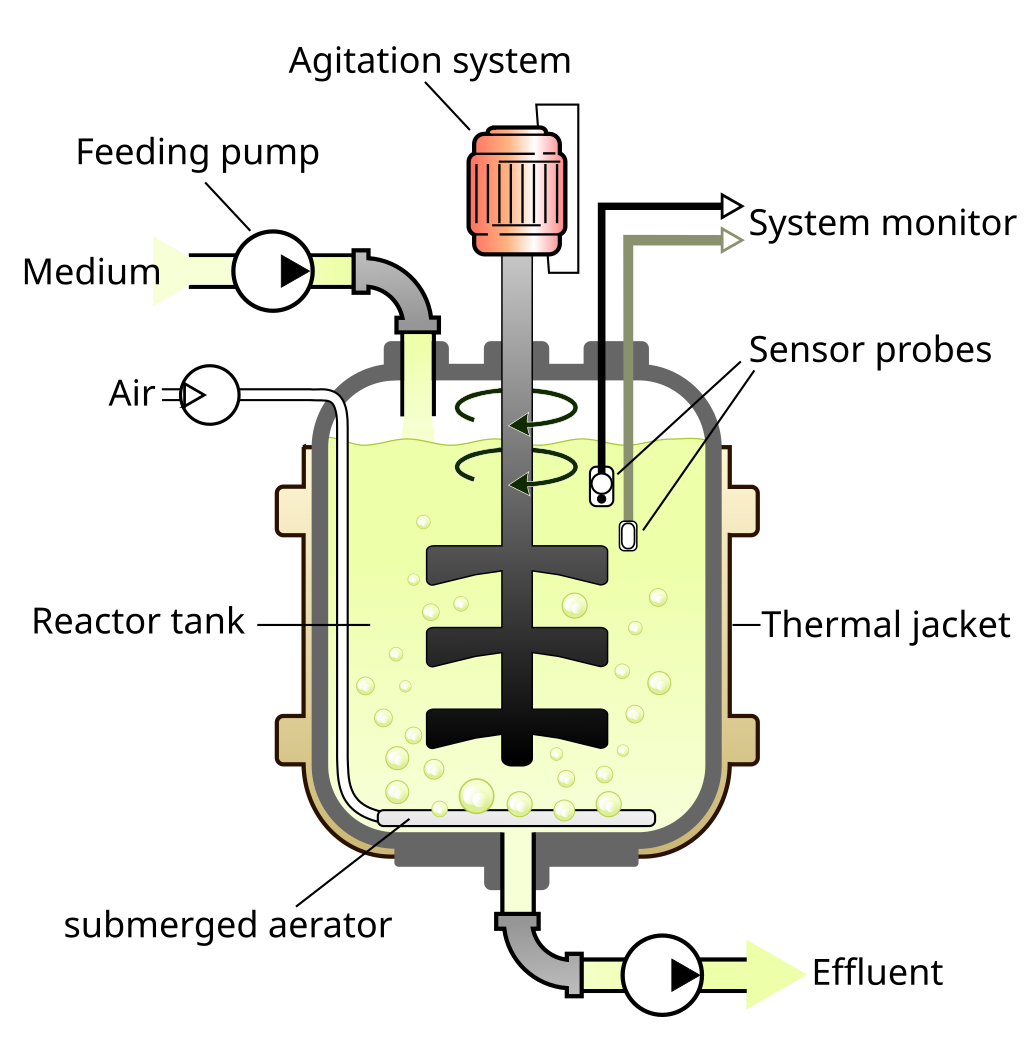
\includegraphics[width=.9\textwidth]{fig/Bioreactor}

          \tiny © Yassine Mrabet, Wikipedia
        }
      \end{center}
    \end{column}
  \end{columns}
\end{frame}

\begin{frame}
  \begin{exampleblock}{Frage}
    Welche Informationen benötigen Sie, um diese Aufgabe zu lösen?
  \end{exampleblock}
\end{frame}

\begin{frame}
  \begin{block}{Verdopplungsrate}
    Under optimal conditions, yeast cells can double their population every 100 minutes.

    \begin{flushright}
      \tiny Wikipedia: Saccaromyces cerevisiæ
    \end{flushright}
  \end{block}

  \pause
  \vspace{5mm}
  
  \begin{tikzpicture}\footnotesize
    \draw [->] (0,0) -- (12.5,0);
    \draw (0,.1)  -- (0,-.1) node[below] {8:00};
    \draw (2,.1) -- (2,-.1) node[below] {9:40};
    \draw (4,.1) -- (4,-.1) node[below] {11:20};
    \draw (6,.1) -- (6,-.1) node[below] {13:00};
    \draw (8,.1) -- (8,-.1) node[below] {14:40};
    \draw (10,.1) -- (10,-.1) node[below] {16:20};
    \draw (12,.1) -- (12,-.1) node[below] {18:00};
    \only<2>{
      \path (1,.3) node {2x};
      \path (3,.3) node {2x};
      \path (5,.3) node {2x};
      \path (7,.3) node {2x};
      \path (9,.3) node {2x};
      \path (11,.3) node {2x};
    }
    \only<3->{
      \path (0.,.1) node[above,iwrred]{1000};
      \path (2.,.1) node[above,iwrred]{2000};
      \path (4.,.1) node[above,iwrred]{4000};
      \path (6.,.1) node[above,iwrred]{8000};
      \path (8.,.1) node[above,iwrred]{16000};
      \path (10.,.1) node[above,iwrred]{32000};
      \path (12.,.1) node[above,iwrred]{64000};
    }
    \only<4>{
      \draw[mygreen] (7,.1) -- (7,-.1) node[below,mygreen] {13:50};
    }
  \end{tikzpicture}

  \pause
  \vspace{5mm}

  \begin{block}{Anfangspopulation}
    Beispiel: Die Population um 8:00 beträgt 1000 Zellen
  \end{block}
  \pause
  \begin{exampleblock}{Frage}
    Wieviele Zellen haben wir um 13:50?
  \end{exampleblock}
\end{frame}

\begin{frame}{Mathematisch etwas allgemeiner und präziser...}
  \begin{itemize}
  \item Anzahlvariable $N$
  \item Zeitvariable $t$ in Minuten, Startzeit $t_0=8:00$, ``Messzeit'' $T=18:00$
  \item Zeitintervalle $I_k = [t_{k},t_{k+1}]$ der Länge $\Delta t = 100 \text{min}$
    
    \vspace{5mm}
  \begin{tikzpicture}\footnotesize
    \draw [->] (0,0) -- (12.5,0);
    \draw (0,.1)  -- (0,-.1) node[below] {8:00};
    \draw (2,.1) -- (2,-.1) node[below] {9:40};
    \draw (4,.1) -- (4,-.1) node[below] {11:20};
    \draw (6,.1) -- (6,-.1) node[below] {13:00};
    \draw (8,.1) -- (8,-.1) node[below] {14:40};
    \draw (10,.1) -- (10,-.1) node[below] {16:20};
    \draw (12,.1) -- (12,-.1) node[below] {18:00};
      \path (0.,.1) node[above,iwrred]{1000};
      \path (1,.3) node {+1000};
      \path (3,.3) node {+2000};
      \path (5,.3) node {+4000};
      \path (7,.3) node {+8000};
      \path (9,.3) node {+16000};
      \path (11,.3) node {+32000};
    \end{tikzpicture}

    \vspace{5mm}
    
  \item Sei $d_k$ der Zuwachs im Intervall $I_k$
    \begin{gather*}
      N(t_{k+1}) = N(t_k) + d_k,
      \qquad N(T) = N(t_0) + \sum_{k=0}^{n-1} d_k.
    \end{gather*}
  \end{itemize}
  \pause
  \begin{exampleblock}{Frage}
    Im Beispiel ist $d_k=N(t_k)$. Wie ändert sich $d_k$ qualitativ, wenn wir die Intervalle halbieren?
  \end{exampleblock}
\end{frame}

\begin{frame}{Halbierung der Intervalle}

  \begin{tikzpicture}\footnotesize
    \draw [->] (0,0) -- (12.5,0);
    \draw (0,.1)  -- (0,-.1) node[below] {8:00};
    \draw (2,.1) -- (2,-.1) node[below] {9:40};
    \draw (4,.1) -- (4,-.1) node[below] {11:20};
    \draw (6,.1) -- (6,-.1) node[below] {13:00};
    \draw (8,.1) -- (8,-.1) node[below] {14:40};
    \draw (10,.1) -- (10,-.1) node[below] {16:20};
    \draw (12,.1) -- (12,-.1) node[below] {18:00};
      \path (0.,.1) node[above,iwrred]{1000};
      \path (1,.3) node {+1000};
      \path (3,.3) node {+2000};
      \path (5,.3) node {+4000};
      \path (7,.3) node {+8000};
      \path (9,.3) node {+16000};
      \path (11,.3) node {+32000};
    \end{tikzpicture}

    \vspace*{4cm}
\end{frame}

\begin{frame}{Riemannsche Summen}
  \begin{itemize}
  \item Es gilt eine Beziehung wie
    $d_k \approx f(t_k)\Delta t$.
  \item Dann können wir für eine beliebige Folge von $n$ Intervallen
    schreiben
    \begin{gather*}
      N(t_n) = N(t_0) + \sum_{k=0}^{n-1} f(t_k) (\Delta t)_k
    \end{gather*}
    \item Wenn wir die Intervalllänge gegen null gehen lassen, bekommen wir ein Integral
  \end{itemize}
  \pause
  \begin{block}{Kontinuumshypothese}
    Für individuelle Hefezellen ist $\Delta t \to 0$ unsinnig, weil sich ab einem Punkt sehr wahrscheinlich keine einzige Zelle in einem Intervall vermehrt.

    \vspace{1ex}

    Wir ersetzen daher die diskrete Anzahl $N(t)$ durch eine
    kontinuierliche Größe $x(t)$ z. B. mit der Einheit Gramm anstelle
    von Stück.
  \end{block}
\end{frame}

\begin{frame}{Integraldarstellung}
  Ersetzen wir $N(t)$ durch $x(t)$ und lassen die Summen konvergieren, so erhalten wir die Darstellung
    \begin{gather*}
      x(T) = x(t_0) + \int_{t_0}^T f(t) \dt.      
    \end{gather*}
  \begin{block}{Instantane Reproduktionsrate $R$}
    Für die Funktion unter dem Integral setzen wir
    \begin{gather*}
      f(t) = R x(t).
    \end{gather*}
    Hier repräsentiert $R$ eine Reproduktionsrate für ein unendlich kleines Zeitintervall.
    %, also
    % \begin{gather*}
    %   R = \lim_{h\to 0} \tfrac{x(t+h)-x(t)}{h}.
    % \end{gather*}
  \end{block}
\end{frame}

\begin{frame}
  Wir erhalten die Darstellung der Funktion $x(t)$ als
  \begin{block}{Volterrasche Integralgleichung}
    \begin{gather*}
      x(t) = x(t_0) + \int_{t_0}^t R x(s) \ds.      
    \end{gather*}    
  \end{block}

  Differenzieren wir auf beiden Seiten ergibt die Darstellung als
  \begin{block}{Differentialgleichung}
    \begin{gather*}
          x'(t) = R x(t)
    \end{gather*}
  \end{block}
\end{frame}

\begin{frame}{Lösungen}
  Aus der Schule ist die Exponentialfunktion bekannt. Es gilt:
  \begin{gather*}
    \tfrac d{dt} e^{Rt} = R e^{Rt}.
  \end{gather*}
  Dies gilt aber auch für alle Funktionen $x(t) = c \,e^{Rt}$ mit einer Konstanten $c$.

  \begin{block}{Anfangswertaufgabe}
    Die Lösungsgesamtheit der Differentialgleichung $x' = Rx$ besteht
    aus allen Funktionen der Form $c\,e^{Rt}$.

    \vspace{1ex}

    Die tatsächliche Lösung erhält man, indem man die Konstante an den Anfangswert $x_0$ angleicht:
    \begin{gather*}
      x_0 = x(t_0) = c e^{Rt_0} \qquad \Rightarrow \qquad c = \frac{x_0}{e^{R t_0}}
    \end{gather*}
  \end{block}
\end{frame}

\begin{frame}{Berechnung von $R$}
  Wenn $\Delta t$ die Zeit zur Verdopplung ist, wie groß ist $R$?

  \vspace{5cm}
  
\end{frame}

\begin{frame}{Einheiten}
  \begin{minipage}{.5\textwidth}
  \begin{itemize}
  \item Wir setzen Einheiten für $t$ und $x$, zum Beispiel
    \begin{gather*}
      t[\text{min}],\qquad x[\text{g}].
    \end{gather*}
  \item Dann hat $x'$ die Einheit $\nicefrac{\text{g}}{\text{min}}$
  \item Wegen
    \begin{gather*}
      R = \frac{x'}{x} \qquad\text{ist}\quad R[\nicefrac1{\text{min}}]
    \end{gather*}
  \end{itemize}    
  \end{minipage}
  \pause
  \begin{block}{Dimensionslose Formulierung}
    Indem man formal durch die Einheiten teilt, werden die Gleichungen
    dimensionslos.

    \vspace{1ex}

    Man kann auch durch charakteristische Größen teilen, um gezielt
    mathematisch einfache Darstellungen zu erhalten.
  \end{block}
\end{frame}

\begin{frame}{Asymptotische Betrachtung}
  \begin{exampleblock}{Frage}
    Was passiert, wenn Sie die Lösung der Wachstumsgleichung für immer
    größere Zeiten, also das Verhalten für $t\to\infty$ betrachten?
  \end{exampleblock}

  \begin{exampleblock}{Frage}
    Was passiert für $t\to\infty$, wenn $R<0$?
  \end{exampleblock}
\end{frame}
%%%%%%%%%%%%%%%%%%%%%%%%%%%%%%%%%%%%%%%%%%%%%%%%%%%%%%%%%%%%%%%%%%%%%% 
%%%%%%%%%%%%%%%%%%%%%%%%%%%%%%%%%%%%%%%%%%%%%%%%%%%%%%%%%%%%%%%%%%%%%%
\subsection{Einige Begriffe}
\frame{\subtoc}
\begin{frame}
  \begin{block}{Differentialgleichung}
    Eine Differentialgleichung ist eine Gleichung, die eine Funktion
    und/oder ihre Ableitungen in Beziehung setzt.
  \end{block}
  \begin{columns}
    \begin{column}[t]{.5\textwidth}
      \begin{block}{Gewöhnliche DGl.}
        Es kommen nur Ableitungen bzgl. einer Variablen vor. Beispiel:
        \begin{gather*}
          x^{(3)}(t) + \sin(t) x'(t) = x^2(t) +t^2
        \end{gather*}
      \end{block}
    \end{column}
    \begin{column}[t]{.5\textwidth}
      \begin{block}{Partielle DGl.}
        Es kommen partielle Ableitungen nach mehreren Variablen vor.
        Beispiel:
        \begin{gather*}
          \partial_t u(t,x) - \partial_{xx} u(t,x) = \sin(x)
        \end{gather*}
      [Nicht in dieser Vorlesung]
      \end{block}
    \end{column}
  \end{columns}
  \pause
  \begin{block}{Ordnung einer Differentialgleichung}
    Die Ordnung einer DGl. ist der Grad der höchsten Ableitung, die in
    der Gleichung vorkommt.
  \end{block}
\end{frame}

\begin{frame}
  \begin{block}{Autonome Differentialgleichungen}
    Eine Differentialgleichung heißt autonom, wenn keiner der Terme
    eine explizite Abhängigkeit von der Zeit hat.
  \end{block}
  \begin{columns}
    \begin{column}[t]{.5\textwidth}
      \begin{block}{Autonom}
        \begin{gather*}
          x' = f(x)
        \end{gather*}
      \end{block}
    \end{column}
    \begin{column}[t]{.5\textwidth}
      \begin{block}{Nicht autonom}
        \begin{gather*}
          x' = f(t,x)
        \end{gather*}
      \end{block}
    \end{column}
  \end{columns}
  \pause Konsequenz: bei autonomen DGln. ist der Startzeitpunkt frei
  verschiebbar, wir wählen oft $t_0 = 0$.
  \begin{exampleblock}{Frage}
    Welche Prozesse führen zu autonomen DGln., welche zu nicht autonomen?
  \end{exampleblock}
\end{frame}

\begin{frame}
  \begin{block}{Homogene Differentialgleichungen}
    Eine Differentialgleichung ist homogen, wenn es keinen Summanden
    gibt, der die Lösungsfunktion nicht enthält. Einen solchen
    Summanden nennt man dann die Inhomogenität.
  \end{block}
  \begin{columns}
    \begin{column}[t]{.5\textwidth}
      \begin{block}{Homogen}
        \begin{gather*}
          x'+ \sin(t) x = 0
        \end{gather*}
      \end{block}
    \end{column}
    \begin{column}[t]{.5\textwidth}
      \begin{block}{Nicht homogen}
        \begin{gather*}
          x'+ \sin(t) x = 5
        \end{gather*}
      \end{block}
    \end{column}
  \end{columns}
  \begin{exampleblock}{Frage}
    Welche Prozesse führen zu homogenen DGln., welche zu nicht homogenen?
  \end{exampleblock}
\end{frame}

%%%%%%%%%%%%%%%%%%%%%%%%%%%%%%%%%%%%%%%%%%%%%%%%%%%%%%%%%%%%%%%%%%%%%%
%%%%%%%%%%%%%%%%%%%%%%%%%%%%%%%%%%%%%%%%%%%%%%%%%%%%%%%%%%%%%%%%%%%%%%
\subsection{Wachstum bei begrenzter Nahrung}
\frame{\subtoc}

\begin{frame}
  \begin{exampleblock}{Frage}
    Was erwarten Sie im Fermenter, wenn Sie im Prozess keine Nahrung
    zuführen? Betrachten Sie vor allem den Fall $t\to\infty$.
  \end{exampleblock}
\end{frame}

\begin{frame}
  \begin{exampleblock}{Frage}
    Was erwarten Sie im Fermenter, wenn Sie im Prozess mit konstanter
    Rate Nahrung zuführen? Betrachten Sie vor allem den Fall
    $t\to\infty$.
  \end{exampleblock}
\end{frame}

\begin{frame}{Modellierung}
  \begin{itemize}
  \item Bisher hatten wir $R$ bei optimalen Bedingungen (Nahrungsmenge
    $F_{\text{opt}}$)
  \item Bei Nahrungszufuhr $F_{\text{opt}}$ ist der Anteil an verfügbarer Nahrung $1-Vx$, wobei $Vx$ der Verbrauch der Hefe ist.
  \item Jetzt setzen wir unter Vereinfachung für die Reproduktionsrate
    \begin{gather*}
      r = R \frac{F}{F_{\text{opt}}} = R (1-Vx)
    \end{gather*}
  \item Wir erhalten die ``logistische Differentialgleichung''
    \begin{gather*}
      x' = rx = R (1-Vx) x.
    \end{gather*}
  \end{itemize}
\end{frame}

\begin{frame}
  \begin{block}{Lösungen}
    \begin{gather*}
      x_c(t) = \frac{e^{Rt}}{V e^{Rt}+c}
    \end{gather*}
  \end{block}
\end{frame}

\begin{frame}{Richtungsfelder}
  \begin{columns}
    \begin{column}[t]{.2\textwidth}
    \begin{gather*}
      x'= (1-x) x
    \end{gather*}
    \begin{exampleblock}{Frage}
      Verhalten für $t\to\infty$
    \end{exampleblock}
    \end{column}
    \begin{column}[t]{.8\textwidth}
      \mbox{}
      
      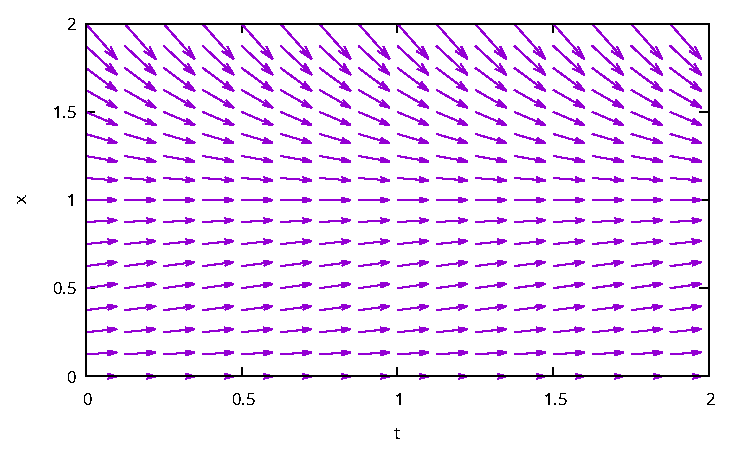
\includegraphics[width=\textwidth]{gnuplot/logistic.pdf}
    \end{column}
  \end{columns}
\end{frame}

\begin{frame}{Negative Startwerte}
  \begin{columns}
    \begin{column}[t]{.2\textwidth}
    \begin{gather*}
      x'= (1-x) x
    \end{gather*}      
    \end{column}
    \begin{column}[t]{.8\textwidth}
      \mbox{}
      
      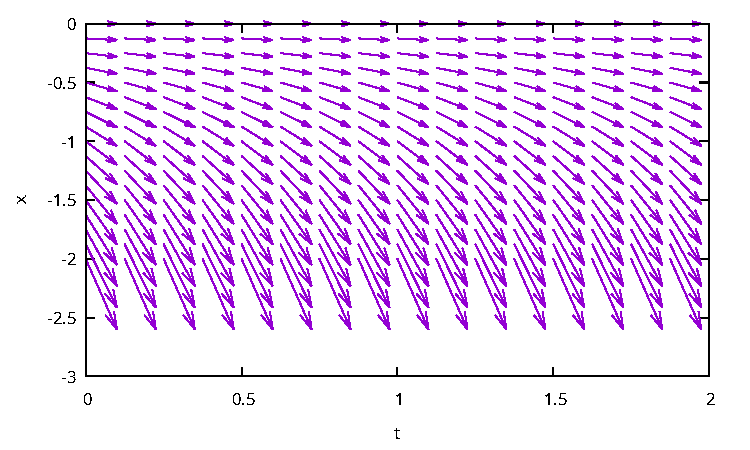
\includegraphics[width=\textwidth]{gnuplot/logisticm.pdf}
    \end{column}
  \end{columns}
\end{frame}

\begin{frame}{Fixpunkte}
  \begin{columns}
    \begin{column}{.1\textwidth}
      \mbox{}
      
      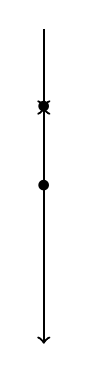
\begin{tikzpicture}[scale=1.]]
        \draw[thick,->] (0,0)  node {$\bullet$} -- (0,1) node {$\bullet$};
        \draw[thick,<-] (0,-2) -- (0,0);
        \draw[thick,->] (0,2) -- (0,1);
      \end{tikzpicture}
    \end{column}
    \pause
    \begin{column}{.9\textwidth}
      Für autonome Gleichungen sind Fixpunkte von hoher Bedeutung. Es gilt:
      \begin{gather*}
        x'(T) = 0 \qquad \Rightarrow \qquad x(t) = 0
        \quad\text{für alle}\quad t>T
      \end{gather*}

      Es gibt
      \begin{itemize}
      \item anziehende Fixpunkte: Richtungspfeile zeigen zum Fixpunkt hin
      \item abstoßende Fixpunkte: Richtungspfeile zeigen vom Fixpunkt weg
      \item gemischte Fixpunkte
      \end{itemize}
    \end{column}
  \end{columns}

\end{frame}


%%%%%%%%%%%%%%%%%%%%%%%%%%%%%%%%%%%%%%%%%%%%%%%%%%%%%%%%%%%%%%%%%%%%%%
%%%%%%%%%%%%%%%%%%%%%%%%%%%%%%%%%%%%%%%%%%%%%%%%%%%%%%%%%%%%%%%%%%%%%%
\subsection{Das Räuber-Beute-Modell}
\frame{\subtoc}

%%%%%%%%%%%%%%%%%%%%%%%%%%%%%%%%%%%%%%%%%%%%%%%%%%%%%%%%%%%%%%%%%%%%%%
%%%%%%%%%%%%%%%%%%%%%%%%%%%%%%%%%%%%%%%%%%%%%%%%%%%%%%%%%%%%%%%%%%%%%%
\subsection{Zusammenfassung und Aufgaben}
\frame{\subtoc}

\begin{frame}{Zusammenfassung}
  \begin{enumerate}
  \item Unter Annahme der Kontinuumshypothese können wir
    Wachtumsprozesse durch Differentialgleichungen
    beschreiben.
  \item Mehrere Spezies führen zu Systemen von DGln.
  \item Diese DGLn. haben unendlich viele Lösungen, was uns eigentlich interessiert, ist die Lösung einer Anfangswertaufgabe (AWA)
  \item Das Ergebnis der eigentlichen Modellierung war die
    Volterrasche Integralgleichung
  \item Wir haben die allgemeine Lösung der DGl. geraten und an den
    Anfangswert angeglichen
  \end{enumerate}
\end{frame}

\section{Berechnung von Lösungen}
\frame{\sectoc}

\section{Qualitative Betrachtungen}
\frame{\sectoc}



\end{document}

%%% Local Variables:
%%% mode: latex
%%% TeX-master: t
%%% End:
